\documentclass[
	12pt,
	a4paper,
	%twoside, % for two pages printing
	pointlessnumbers, % Kein Punkt nach der letzten Ziffer
	bibtotoc, % Literatur ins Inhaltsverzeichnis
	halfparskip+,
	listof=totocnumbered
	]{scrartcl}

% Packages
\usepackage[utf8]{inputenc}
\usepackage[T1]{fontenc}
\usepackage[english]{babel}
\usepackage{pdfpages}

% Math
\usepackage{amsmath}
\usepackage{amsfonts}   
\usepackage{amssymb}
\usepackage{amsthm}
\usepackage{nicefrac}
\usepackage{siunitx}
\usepackage{xstring}

\usepackage[ruled,vlined,english,linesnumbered]{algorithm2e}

% Tabellen
\usepackage{rotating}
\usepackage{multirow}

% Rahmen
\usepackage{fancybox}
\usepackage{framed}

% Layout
%\usepackage{geometry}
\usepackage{listings}
\usepackage{makeidx}
\usepackage{pdflscape}
\usepackage{thmtools}
\usepackage{multicol}
\usepackage[ruled,vlined,english,linesnumbered]{algorithm2e} % Algorithmenpacket
\usepackage{fancyhdr} % Header
\usepackage[german, plain]{fancyref}
\usepackage[font=small, format=plain, labelfont=bf, up, textfont=it, up]{caption}
\usepackage{xcolor,colortbl}
\usepackage{booktabs}


\renewcommand{\arraystretch}{1.25}
\newcommand{\bigcell}[2]{\begin{tabular}{@{}#1@{}}#2\end{tabular}}


% Grafik
\usepackage{graphicx}
\usepackage{float}
\usepackage{wrapfig}
\usepackage{tikz}
\usetikzlibrary{matrix, chains, positioning, automata, arrows, calc, snakes, patterns, decorations, decorations.pathmorphing, decorations.pathreplacing, decorations.markings, intersections, shadows, shapes.geometric, trees}
\usepackage{fix-cm}
\usepackage{pgfplots}
\usepackage{overpic}
\usepackage[american,cuteinductors,smartlabels]{circuitikz}
\usepackage{caption}
\usepackage{subcaption}
\usepackage{tikz-timing}
\usepackage{pgf-umlsd}

%\usepgfplotslibrary{external}
%\tikzexternalize{bachelorthesis}

% Bibliography
\usepackage[style=numeric]{biblatex}




\usepackage[
    %nativepdf, 
    pagebackref=false,
    draft=false,
    pdfpagelabels=false,
    pdfstartview=FitH,
    pdfstartpage=1,
    bookmarks=true,
    pdftitle={Decision Trees},
    pdfsubject={An Introduction},
    pdfkeywords={decision tree, dt, decision, tree},
    unicode=true
]{hyperref} 


\usepackage{bookmark}


\newcommand{\kreis}[1]{\unitlength1ex\begin{picture}(2.5,2.5)%
\put(0.75,0.75){\circle{2.5}}\put(0.75,0.75){\makebox(0,0){#1}}\end{picture}}

\renewbibmacro*{cite}{%
  \textbf{% ADDED
  \printtext[bibhyperref]{%
    \printfield{prefixnumber}%
    \printfield{labelnumber}%
    \ifbool{bbx:subentry}
      {\printfield{entrysetcount}}
%      {}}}% DELETED
      {}}}}% ADDED




% Definitions

% matlabtikz bugfix
\newlength\figureheight 
\newlength\figurewidth 




% Headerübersicht

\pagestyle{plain} %eigener Seitenstil
\fancyhf{} %alle Kopf- und Fußzeilenfelder bereinigen
\fancyhead[LO]{\nouppercase{\textbf{\sffamily \leftmark}}} %Kopfzeile links
\fancyhead[CO]{} %zentrierte Kopfzeile
\fancyhead[RO]{\nouppercase{\sffamily \rightmark}} 

\fancyhead[LE]{\nouppercase{\sffamily \rightmark}} %Kopfzeile links
\fancyhead[CE]{} %zentrierte Kopfzeile
\fancyhead[RE]{\nouppercase{\textbf{\sffamily \leftmark}}}

%Kopfzeile rechts: 
\includegraphics[scale=0.025]{graphics/layout/faulogo.png}
\renewcommand{\headrulewidth}{0.4pt} %obere Trennlinie
\fancyfoot[LE]{\thepage} %Seitennummer
\fancyfoot[RO]{\thepage} %Seitennummer
%\renewcommand{\footrulewidth}{0.4pt} %untere Trennlinie

\pagestyle{fancy}

%\renewcommand{\partmark}[1]{\markboth
%  {\thepart. #1}{}}
%
%\renewcommand{\chaptermark}[1]{\markright
%  {\thechapter.\ #1}}
%
%\renewcommand{\sectionmark}[1]{}


%\let\chapter\section % Behebung für Algorithm2e

\addto\captionsUKenglish{%
    \renewcommand{\contentsname}{Table of Contents}
}


% Farben

\definecolor{faugray}{gray}{0.5} % die Farbe grau wird definiert
\definecolor{light-gray}{gray}{0.65}

\definecolor{fauyellow}{cmyk}{0.01, 0.08, 0.92, 0.01}
\definecolor{faublue}{cmyk}{0.94, 0.63, 0.03, 0.05}
\definecolor{faured}{cmyk}{0.02, 0.94, 0.90, 0.06}
\definecolor{fauorange}{cmyk}{0.01, 0.57, 0.91, 0.02}
\definecolor{faucoolgray}{cmyk}{0.55, 0.31, 0.25, 0.02}
\definecolor{faugreen}{cmyk}{0.83, 0.03, 0.93, 0.06}





% Index
\makeindex



% Stildefinition für listings
\lstdefinestyle{fau} {
	basicstyle		= \ttfamily\small,
	identifierstyle	= \ttfamily\normalsize,
	stringstyle		= \ttfamily\small\color{faured},
	commentstyle	= \ttfamily\small\color{faugreen},
	keywordstyle	= \ttfamily\small\color{faublue},
	columns			= fullflexible,
	showstringspaces= false,
	emphstyle 		= \color{fauorange},
	frame			= single,
	morekeywords	= {REFERENCES, DATETIME},
	emph			= {Michi},
	framesep 		= 15pt,
	rulesep			= 15pt,
	framerule		= 0.25pt,
	captionpos		= b,
	%linewidth		= 0.75\textwidth,
	xleftmargin 	= 15pt,
	xrightmargin	= 15pt,
	aboveskip		= 15pt,
	belowskip		= 15pt
 }
 
\lstdefinelanguage[Objective]{C}[GNU99]{C}
  {morekeywords={@catch,@class,@encode,@end,@finally,@implementation,%
      @interface,@private,@protected,@protocol,@public,@selector,%
      @synchronized,@throw,@try,BOOL,Class,IMP,NO,Nil,SEL,YES,_cmd,%
      bycopy,byref,id,in,inout,nil,oneway,out,self,super,%
      % The next two lines are Objective-C 2 keywords.
      @dynamic,@package,@property,@synthesize,readwrite,readonly,%
      assign,retain,copy,nonatomic%
      },%
   moredirectives={import}%
  }%

\lstdefinelanguage[GNU99]{C}[99]{C}
  {morekeywords={asm,__asm__,__extension__,typeof,__typeof__}%
  }%

\lstdefinelanguage[99]{C}%
  {morekeywords={_Bool,_Complex,_Imaginary,auto,break,case,char,%
      const,continue,default,do,double,else,enum,extern,float,for,%
      goto,if,inline,int,long,register,restrict,return,short,signed,%
      sizeof,static,struct,switch,typedef,union,unsigned,void,volatile,%
      while},%
   sensitive,%
   morecomment=[s]{/*}{*/},%
   morecomment=[l]//,%
   morestring=[b]",%
   morestring=[b]',%
   moredelim=*[directive]\#,%
   moredirectives={define,elif,else,endif,error,if,ifdef,ifndef,line,%
      include,pragma,undef,warning}%
  }[keywords,comments,strings,directives]%




\declaretheoremstyle[
    spaceabove=1em, spacebelow=2em,
    headfont=\normalfont\bfseries,
    notefont=\normalfont\bfseries, notebraces={(}{)},
    bodyfont=\normalfont,
    shaded={bgcolor=gray!5, rulecolor=black, rulewidth=0.5pt, margin=0.5em}
]{defstyle}


\declaretheorem[style=defstyle]{definition}
\declaretheorem[style=defstyle, name=Remark, numbered=no]{remark}
\declaretheorem[style=defstyle, name=Discussion, numbered=no]{discussion}
%\declaretheorem[numbered=no]{proof}
\declaretheorem[name=Example, numbered=no]{example}


\newcommand{\nicequote}[2]
{
    \begin{center}{\Huge \bfseries ``}
        \begin{minipage}[t]{0.8\textwidth} \itshape
            #2 
            \begin{flushright} \vspace*{-1em}
                 -- #1
            \end{flushright}
        \end{minipage} \, {\Huge \bfseries ''} 
    \end{center}
}

\newcommand{\situationTable}[5]
{
    #1 & #2 \\ 
}

\pgfplotsset{
  compat=newest,
  xlabel near ticks,
  ylabel near ticks
}





\bibliography{content/bibliography}


\begin{document}


%\includepdf[pages=-]{content/titlepage.pdf}

\title{Introduction to Decision Trees}



\begin{titlepage} 
\thispagestyle{empty}


%Sustainable Energy by Benni from The Noun Project

\begin{center}
    {\fontsize{60}{60} \bfseries \textsf{Decision Trees}}\\[1em]
        
    \noindent\rule{\textwidth}{0.5pt} \\[1em]
    {\Large \textsf{An Introduction} } \\[4em]
    %\noindent\rule{\textwidth}{0.5pt} \\[3em]
    
    
\includegraphics[width=0.35\textwidth]{content/decisiontree}
    
    \vspace{5em}

    {\sffamily \large \bfseries  Seminar paper for the course \textit{Artificial Intelligence} (KISEM)}\\[3em]


    {  \normalsize 
        Michael Dorner \\[2em]
        
        \today

    } 
\end{center}

\end{titlepage}


\newpage

\renewcommand{\contentsname}{Table of Content}
\tableofcontents
\vfill


\newpage


% Content

\section{Introduction}


\subsection{What is a decision tree?} \label{whatisadecisiontree}
A business student with only a very few programming skills shall develop a simple algorithm for sorting three elements $A, B, C$. He decides to divide this problem in smaller subproblems. First he wonders if $A$ is smaller then $B$. In the second step it is interesting if $B$ is smaller then $C$. If $A<B$ and $B<C$ then $A<B<C$. But if $B$ is not greater then $C$, then a third question is relevant: Is $A<C$? 

His head is spinning. Maybe solving this problem graphically is a better idea. He draws a node for each question and an edge for each answer. All leafs represent the correct order. Figure \ref{fig:sortingtree} shows the resulting graph:

\begin{figure}[!h]
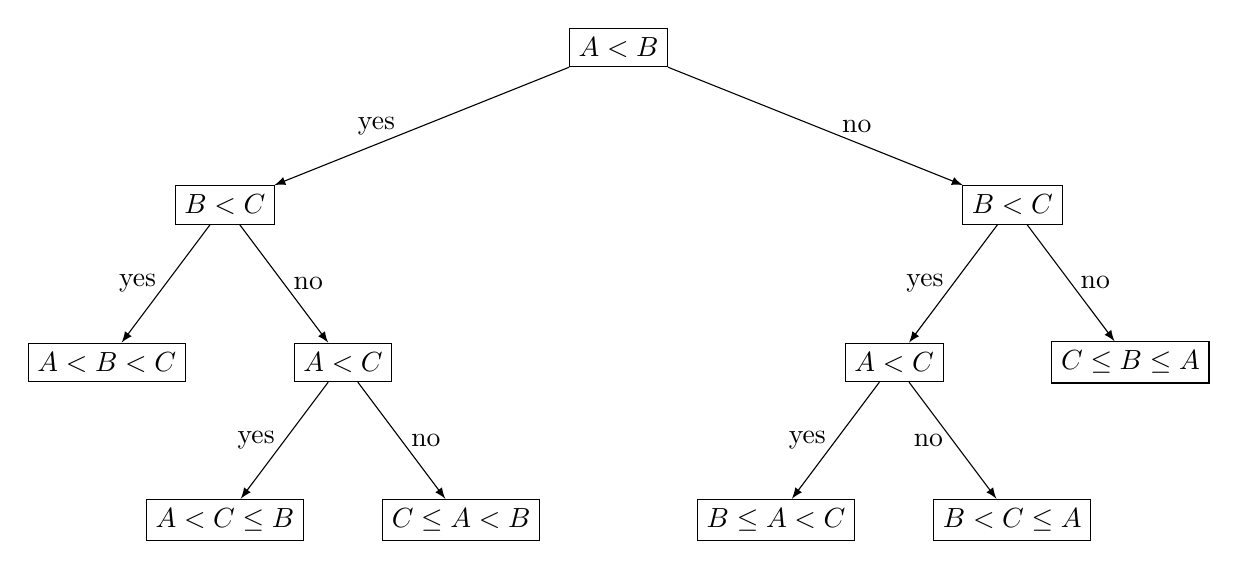
\begin{tikzpicture}[edge from parent/.style={draw,-latex},
level distance=2cm,
level 1/.style={sibling distance=10cm},
level 2/.style={sibling distance=3cm}]
\tikzstyle{every node}=[rectangle,draw]    
\node (Root) {$A < B$}
child {
    node {$B < C$}    
    child { 
        node {$A < B < C$} 
        edge from parent node[left,draw=none] {yes}
    }
    child { 
        node {$A < C$} 
        child {
            node {$A < C \leq B$}
            edge from parent node[left,draw=none] {yes}
        }
        child {
            node {$C \leq A < B$}
            edge from parent node[right,draw=none] {no}
        }
        edge from parent node[right,draw=none] {no}
    }
    edge from parent node[left,draw=none] {yes $\;$}
}
child {
    node {$B < C$}
    child { 
        node {$A < C$}     
        child {
            node {$B \leq A < C$}
            edge from parent node[left,draw=none] {yes}
        }   
        child {
            node {$B < C \leq A$}
            edge from parent node[left,draw=none] {no}
        }     
        edge from parent node[left,draw=none] {yes}
    }
    child { 
        node {$C \leq B \leq A$} 
        edge from parent node[right,draw=none] {no}
    }
    edge from parent node[right,draw=none] { $\;$ no}
};
\end{tikzpicture}
\caption{A decision tree for sorting three values.}
\label{fig:sortingtree}
\end{figure}

Without further knowledge the student created his first decision tree.

For a right decision two or three if-statements are necessary. So a Python program could look like listing \ref{lst:sort1}.

\newpage

\begin{lstlisting}[style = fau, language = Python, caption={[A Python implementation of a decision tree for sorting three elements]A Python implementation of a decision tree for sorting three elements $A, B, C$},label=lst:sort1]
def sort1(A, B, C):
	if (A < B):
		if (B < C):
			return [A, B, C]
		else:
			if (A < C):
				return [A, C, B]
			else:
				return [C, A, B]
	else:
		if (B < C):
			if (A < C):
				return [B, A, C]
			else:
				return [B, C, A]
		else:
			return [C, B, A]

print( sort1(9,-2,0) ) # >> [-2, 0, 9]
print( sort1(2,0,0) )  # >> [0, 0, 2]
\end{lstlisting}

\begin{remark}
    The Python if-statement syntax implies the tree structure in a vertical form, too.      
\end{remark}

Another way of formatting if-clauses represents a rule set which are first order logical expressions:  
    \begin{lstlisting}[style = fau, language = Python, caption={A Python reimplementation of the decision tree given in listing \ref{lst:sort1} as a set of first order logical rules},label=lst:sort2]
def sort2(A, B, C):
	if (A < B) and (B < C) : return [A, B, C]
	if (A < B) and not (B < C) and (A < C): return [A, C, B]
	if (A < B) and not (B < C) and not (A < C): return [C, A, B]
	if not (A < B) and (B < C) and (A < C): return [B, A, C]
	if not (A < B) and (B < C) and not (A < C): return [B, C, A]
	if not (A < B) and not (B < C) : return [C, B, A]
\end{lstlisting}

Unsurprisingly, we get six rules for $3! = 6$ different combinations and the same results as in the algorithm \texttt{sort1}. 


This introductory example shows four important properties: Decision trees
\begin{enumerate}
    \item work very well for classification and data mining.
    \item are intuitive and self-explanatory.
    \item are easy to implement.
    \item can be even used by business students.
\end{enumerate}

\begin{remark}
    Decision trees are used to model all comparison sorts like mergesort or quicksort. The reader may notice that the decision tree in figure \ref{fig:sortingtree} represents the insertion sort algorithm \cite[p. 208]{cormen2001introduction}. 
\end{remark}





\section{Theory of Decision Trees}

In this section a (computer) scientific base for the informal introduction of decision trees shall be given. As mentioned in the introduction a basic knowledge in graph theory, machine learning and computer science in general is assumed.


\subsection{Definitions}

\begin{definition}
A \textbf{tree} is a directed, connected graph with one root node. Every other node has a single predecessor (\textbf{parent}) and no or more successors (\textbf{children}). Nodes without successors are called \textbf{leaves}. All nodes are connected by \textbf{edges}. The \textbf{depth} of a node is the number of edges on the path to the root. The \textbf{height} of the whole tree is the number of edges on the longest path from the root to any leaf. 
\end{definition}

\begin{remark}
This very rough definition focussed on trees shall not hide the fact that graph theory is complex and enormous mathematical field. For a deeper look e.g. \cite{cormen2001introduction} is recommended.
\end{remark}

\begin{definition}
A \textbf{decision tree} is a tree with following equivalents:
\begin{center}
\begin{tabular}{l|l} 
    \textbf{Tree} &  \textbf{Decision tree equivalent} \\ \hline
    Root & Initial decision node  \\ 
    Node & Internal decision node for testing on an attribute  \\ 
    Edge & Rule to follow \\ 
    Leaf & Terminal node represents the resulting classification 
\end{tabular}
\end{center}
\end{definition}

As mentioned in subsection \ref{taxonomy}, machine learning is a set of algorithms that extract models representing patterns from data and then evaluate those models. Let us define four relevant terms, which are important for understanding the following algorithms descriptions: instance, attribute, class, and dataset:

\begin{definition}
    The input of a machine learning algorithm consists of a set of \textbf{instances} (e.g. rows, examples or observations). Each instance is described by a fixed number of \textbf{attributes} (i.e. columns), which are assumed to be either nominal or numeric, and a label which is called \textbf{class} (in case of a classification task). The set of all instances is called \textbf{dataset}.
\end{definition}

Following this definition we get a table containing the dataset: Each decision becomes an attribute (all binary relations), all leaves are classes, while each row represents an instance of the dataset (see table \ref{tab:decisiontable}).

\begin{table}[!h] \centering
\begin{tabular}{|l| l l l |l|} \hline
    \textbf{Instance} & \multicolumn{3}{c|}{\textbf{Attribute}} & \multicolumn{1}{c|}{\textbf{Class}}\\ 
    & $A<B$ & $B<C$ & $A<C$ &  \\ \hline
    1 & yes & yes & yes & $A < B < C$ \\ 
    2 & yes & yes & no & $A < B < C$ \\
    3 & yes & no & yes & $A < C \leq B$ \\
    4 & yes & no & no & $C \leq A < B$ \\
    5 & no & yes & yes & $B \leq A < C$ \\ 
    6 & no & yes & no & $B < C \leq A$ \\
    7 & no & no & yes & $C \leq B \leq A$ \\
    8 & no & no & no & $C \leq B \leq A$ \\ \hline
\end{tabular}
\caption{Dataset table for the sorting example from subsection \ref{whatisadecisiontree}}
\label{tab:decisiontable}
\end{table}

Normally, the transformation is vice versa: the data is collected in table form (e.g. databases) and a decision tree has to be generated. 

The reason why there are now eight instead of six classes is simple: it does not matter for instances 1, 2 and 7, 8, if $A<B$ or not; the result is the same class. This effect of removing irrelevant branches of a tree is called pruning and is also part of this paper (see \ref{treepruning}). 


\newpage

\subsection{Decision Tree Learning}

In this subsection the question how to generate a decision tree from a given dataset in general shall be answered.

A founding idea of tree-based classification is based in the Concept Learning System \cite{quinlan1986induction}.
All algorithms introduced in the next section are based on a simple but very powerful algorithm called TDIDT which stands for \textit{Top-Down Induction of Decision Trees} \cite{quinlan1986induction}. This algorithm framework consists of two methods, growing and pruning a decision tree, which are introduced in the next two pseudocode listings and follows the idea of divide and conquer \cite[p. 33]{cormen2001introduction}. 

\begin{remark}
    $\sigma$ is the relational operator for selection. See e.g. \cite[p. 145]{rob2008database} for further operators and more detailed information. 
\end{remark}

 
\begin{algorithm}
\SetKwInOut{Input}{Input}
\SetKwInOut{Output}{Output}
\SetKwFunction{treePruning}{treePruning}
\SetKwFunction{treeGrowing}{treeGrowing}
\SetKwFunction{stoppingCriterion}{stoppingCriterion}
\SetKwFunction{splittingCriterion}{splittingCriterion}
\Input{Training set $X$, attribute set $A$, target feature $y$}
\Output{Decision tree}
\BlankLine
Create a new tree $T$ with a single root node.\\
\eIf{\stoppingCriterion{$X$}}{
    Mark $T$ as a leaf with the most common value in $X$ as a label.
}{
    $\forall a_i \in A$ find \textcolor{faured}{$a$} that obtain the best \splittingCriterion{$a_i, X, y$}.\\
    Label $n$ with $a$.\\
    \For{each outcome \textcolor{faublue}{$v_i$} of \textcolor{faured}{$a$}}{
        Set subtree \textcolor{faugreen}{$t_i$} = \treeGrowing{$\sigma_{a=v_i}X, A, y$}. \\
        Connect the root node of $n_t$ to the subtree \textcolor{faugreen}{$t_i$} with an edge that is labelled as \textcolor{faublue}{$v_i$}.
    }
}
\Return{\treePruning{$S, T, y$}}
\caption{Tree Growing \texttt{treeGrowing}}
\end{algorithm}

\begin{algorithm}
\SetKwInOut{Input}{Input}
\SetKwInOut{Output}{Output}
\SetKwFunction{pruned}{pruned}
\Input{Training set $X$, tree to be pruned $T$, target feature $y$}
\Output{Decision tree}
\BlankLine
\Repeat{$t = \emptyset$}{
      Select a node $n$ in $T$ such that pruning this node $n$ maximally improves some evaluation criterions. \\
    \If{$n \neq \emptyset$}{
        $T = $ \pruned{$T, n$}
    }
}
\Return{$T$}
\caption{Tree Pruning \texttt{treePruning}}
\end{algorithm}


A simplified decision tree \ref{fig:frameworktree} created by this algorithmic framework shall clarify how it works. The colors correspond to the variables in the pseudocode.

\begin{figure}[!h] \centering
\begin{tikzpicture}[
    level distance=2cm,
    level 1/.style={sibling distance=2.5cm},
    level 2/.style={sibling distance=4cm},
    leaf/.style={isosceles triangle,dashed,shape border rotate=90,isosceles triangle stretches=true, minimum height=20mm,minimum width=20mm,inner sep=0,yshift={-20mm}}]
\tikzstyle{every node}=[rectangle,draw]    
\node (Root) {\textcolor{faured}{$a$}}
child[child anchor=north] { 
    node[leaf] {\textcolor{faugreen}{$t_1$}}
    edge from parent node[left,draw=none] {\textcolor{faublue}{$v_1\;$}}
}
child[child anchor=north] { 
    node[leaf] {\textcolor{faugreen}{$t_2$}}
    edge from parent node[right,draw=none] {\textcolor{faublue}{$v_2$}}
}
child[child anchor=north] { 
    node[leaf, text height=1.5em] {$\dots $}
    edge from parent node[right,draw=none] {$\dots$}
}
child[child anchor=north] { 
    node[leaf] {\textcolor{faugreen}{$t_n$}}
    child[grow=right, xshift={10mm}] {
        node[draw=none]{Subtrees}
        edge from parent[draw=none]
        child[grow=up, yshift={7.5mm}] {
            node[draw=none]{Values of \textcolor{faured}{$a$}}  
            edge from parent[draw=none]
            child[grow=up, yshift={-7.5mm}] {
                node[draw=none]{Best attribute in $A$}  
                edge from parent[draw=none]
            } 
        }    
    }
    edge from parent node[right,draw=none] {\textcolor{faublue}{$v_n$}}
}
;
\end{tikzpicture}
\caption{The basic structure of a decision tree created by the algorithmic framework.}
\label{fig:frameworktree}
\end{figure}

\newpage


\section{Summary \& Conclusion}

\subsection{Applications}

Decision trees have a wide field of applications. In this subsection some examples of the applications are listed.

\begin{description}
    \item[Astronomy] \cite{salzberg1995decision} applied decision tree learning to the task of distinguishing between stars and cosmic rays in images collected by the Hubble Space Telescope.
    %\item[Library] In [26], decision trees are developed that predict the future use of books in a library.
    \item[Chemistry] The relationship between the research on octane (ROC) number and the molecular substructures were explored in the paper \cite{blurock1995automatic}.
    \item[Medicine] In \cite{vlahou2003diagnosis} decision trees are applied for the diagnosis of the ovarian cancer.     
    \item[Economy] The results of the research project on decision trees used in stock trading was published in \cite{wu2006effective}.
    \item[Geography] \cite{lagacherie1997addressing} used classification trees to predict and correct errors in topographical and geological data.
\end{description}



\subsection{Programming Example}

In the programming example a decision tree induction algorithm was implemented in the programming language Python. The focus during the development was on readability and understanding, less on performance and software architecture. 

Two splitting criterions are implemented: Information and Gini gain (ID3 and CART). Also a basic pruning algorithm can be used, which uses a threshold for the pruning decision (see subsection \ref{stoppingcriterionimpl} for the idea of stopping criterion). The decision tree itself is implemented as binary tree and does not support regression analysis.

Two examples are enclosed: Tuberculosis/pneumonia and fish iris classification. Both are from real world, while the first example consists of only a handful instances due to the fact that this example was calculated completely by hand in the presentation. The second example origins from Matlab demo files. 

The code is well commented and has a demo application for each example. 



\subsection{Summary}

In the scope of this paper, a small introduction to decision trees was given. The introductory example showed the working principle and advantages of decision trees. An overview of machine learning approaches helped to see the bigger picture.  

The theory part started with some necessary definitions which are used in the following parts. The basic top-down induction of decision trees algorithm was introduced and the options for improving this framework were described mathematically.

Four decision tree algorithms were selected and presented to the reader: CHAID, ID3, CART, and C4.5. All facts from the previous sections were compared and traded off one against the other. Due to the limited scope of this seminar paper some parts were not considered in detail, but a small outlook on these interesting topics is given.

The last part shows some examples where decision trees find their application in the real world and how many-faceted this field is. The programming example with a small code documentation completes the picture of decision trees. 











\setcounter{section}{0}
\renewcommand{\thesection}{\Alph{section}}



\newpage

\section{Bibliography}
%\addcontentsline{toc}{section}{Bibliography}
\printbibliography[heading=none]


\end{document}



